\documentclass{article}

\usepackage[eandd]{neurips_2026}
\usepackage[utf8]{inputenc}
\usepackage[T1]{fontenc}
\usepackage{hyperref}
\usepackage{url}
\usepackage{booktabs}
\usepackage{amsfonts}
\usepackage{amsmath}
\usepackage{amssymb}
\usepackage{microtype}
\usepackage{xcolor}
\usepackage{graphicx}

\newcommand{\framework}{SpecLens-RL}

\title{\framework: A Compact Benchmark and Evaluation Protocol for Diagnosing Specification Failures in Reinforcement Learning}
\author{Anonymous Authors}

\begin{document}

\maketitle

\begin{abstract}
We present \framework, a compact benchmark and evaluation protocol for
diagnosing specification failures in reinforcement learning. Rather than
proposing a new optimizer, \framework defines a task tuple that separates proxy
reward, hidden true objective, corruption channels, monitor channels,
distribution shift, and policy family. We instantiate that tuple in three
symbolic environments and evaluate it under strict artifact and leakage rules.
Across all three tasks, proxy-trained policies diverge sharply from oracle
policies on the hidden objective; SensorTamper-v0 additionally exposes a
behaviorally active corruption channel whose removal collapses the learned
proxy exploit; and proxy-only monitor evaluation shows that valid
leakage-cleared monitor evidence is possible but narrow, because only
SensorTamper-v0 yields a nondegenerate hack-label mix under the current
protocol. The result is a compact benchmark for studying reward
misspecification, tampering, and the limits of monitorability claims under
controlled compute budgets.
\end{abstract}

\section{Introduction}
Reinforcement learning agents are usually optimized against a proxy reward while
being judged, implicitly or explicitly, against a broader intended objective.
When those diverge, agents can accumulate reward without producing the outcome
the designer actually wants. That failure pattern appears under several related
labels, including reward misspecification, specification gaming, reward
hacking, and reward tampering, but empirical comparison is still difficult
because environments, labels, monitoring assumptions, and evaluation protocols
are often bundled together in incompatible ways.

\framework takes a diagnosis-first position. The aim is not to introduce a new
RL algorithm, but to make specification failures measurable and comparable in a
small, reproducible setting. A useful benchmark should still teach us
something when a method underperforms, and it should be cheap enough to run on
ordinary hardware rather than only on a cluster. Those constraints matter for
safety evaluation because they encourage explicit task definitions, inspectable
labels, and conservative claims.

We formalize a specification-diagnostic task as
\[
T = (M, R_p, J_t, C, M_{\mathrm{mon}}, \Delta, \Pi),
\]
where $M$ is the underlying MDP or POMDP, $R_p$ is the proxy reward used for
learning, $J_t$ is the hidden true objective used for evaluation, $C$ is the
corruption or tampering channel family, $M_{\mathrm{mon}}$ is the monitor
observation channel, $\Delta$ is the distribution-shift family, and $\Pi$ is
the policy or training family considered. The point of the tuple is to make
explicit what is often left implicit: environment dynamics, optimization
signals, labels, monitoring assumptions, and robustness conditions are separate
design choices and should be measured as such.

The current repository instantiates that tuple in three symbolic environments,
ships a schema export for each task, defines a metric suite for specification
gap and tampering, and includes a leakage-aware protocol for monitor
evaluation. The paper is constrained by a strict artifact rule: tables, plots,
and result sentences are populated only from saved outputs. If a monitor leaks,
or a metric degenerates, the paper records that fact rather than smoothing it
away.

The strongest honest empirical takeaway is narrow but useful. Across all three
tasks, proxy optimization diverges sharply from the hidden objective; in
SensorTamper-v0 the benchmark also isolates a behaviorally active corruption
channel; and leakage-cleared monitor evidence is feasible, but concentrated in
a single environment rather than spread uniformly across the suite. That is a
good fit for a workshop paper about evaluation methodology: \framework is a
compact diagnostic object for future work on reward misspecification,
tampering, and monitorability rather than a claim of broad safety coverage.

\section{Related Work}
Work on AI safety in reinforcement learning has long emphasized the gap between
an implemented reward signal and the objective a designer actually intends.
\citet{amodei2016concrete} catalogued concrete failure modes including reward
hacking and scalable oversight, while AI Safety Gridworlds demonstrated the
value of compact environments for studying such failures under controlled
conditions \citep{leike2017ai}.

Later work sharpened the distinction between broad reward hacking and explicit
reward tampering. Everitt et al.\ analyze tampering incentives with causal
influence diagrams \citep{everitt2021reward}, while Skalse et al.\ characterize
reward hacking as divergence between proxy and true objectives rather than a
grab-bag of anecdotes \citep{skalse2022rewardhacking}. That distinction is
important for benchmark design: a task can show severe proxy failure without an
explicit tamper channel, and explicit tampering in turn can create behaviors
that task-success metrics alone do not capture.

Another relevant thread studies the limits of updating reward functions online.
Even when the reward process is itself adaptive, agents can manipulate weak
oversight or the reward-learning loop \citep{armstrong2020pitfalls}. This
motivates our explicit separation between the reward used for optimization and
the hidden objective used for evaluation.

Procedural generalization work likewise matters here. Layout and nuisance
variation can distinguish brittle reward exploitation from more robust
strategies \citep{cobbe2020leveraging}. In \framework, shift is therefore part
of the task definition rather than an optional stress test. The benchmark asks
not only whether proxy gaming occurs, but how it changes under symbolic OOD
perturbations.

Our contribution is closest to the intersection of these threads: small
model-organism safety environments, formal treatments of reward hacking and
tampering, and benchmark design for robustness. \framework contributes a
compact synthesis centered on explicit task structure, metric discipline, and
leakage-aware monitoring rather than a new optimization technique.

\section{Task Tuple and Evaluation Protocol}
\subsection{Task Tuple}
We define a specification-diagnostic task as
\[
T = (M, R_p, J_t, C, M_{\mathrm{mon}}, \Delta, \Pi).
\]
Each term carries a specific role.

\paragraph{Environment dynamics.}
$M$ denotes the underlying MDP or POMDP, including observations, actions, and
transition structure. In this benchmark, $M$ is always symbolic and CPU-fast.

\paragraph{Optimization and evaluation.}
$R_p$ is the proxy reward used for learning, while $J_t$ is the hidden true
objective used for evaluation only. The gap between them is the central object
of measurement.

\paragraph{Corruption, monitoring, and shift.}
$C$ denotes corruption or tampering channels, $M_{\mathrm{mon}}$ denotes the
observation channel available to an external monitor, and $\Delta$ denotes the
family of OOD perturbations used to probe robustness.

\paragraph{Policy family.}
$\Pi$ denotes the learning family considered. We keep $\Pi$ deliberately small:
standard PPO trained on proxy reward, plus an oracle PPO baseline trained on
the hidden objective for diagnosis only.

\begin{figure*}[t]
\centering
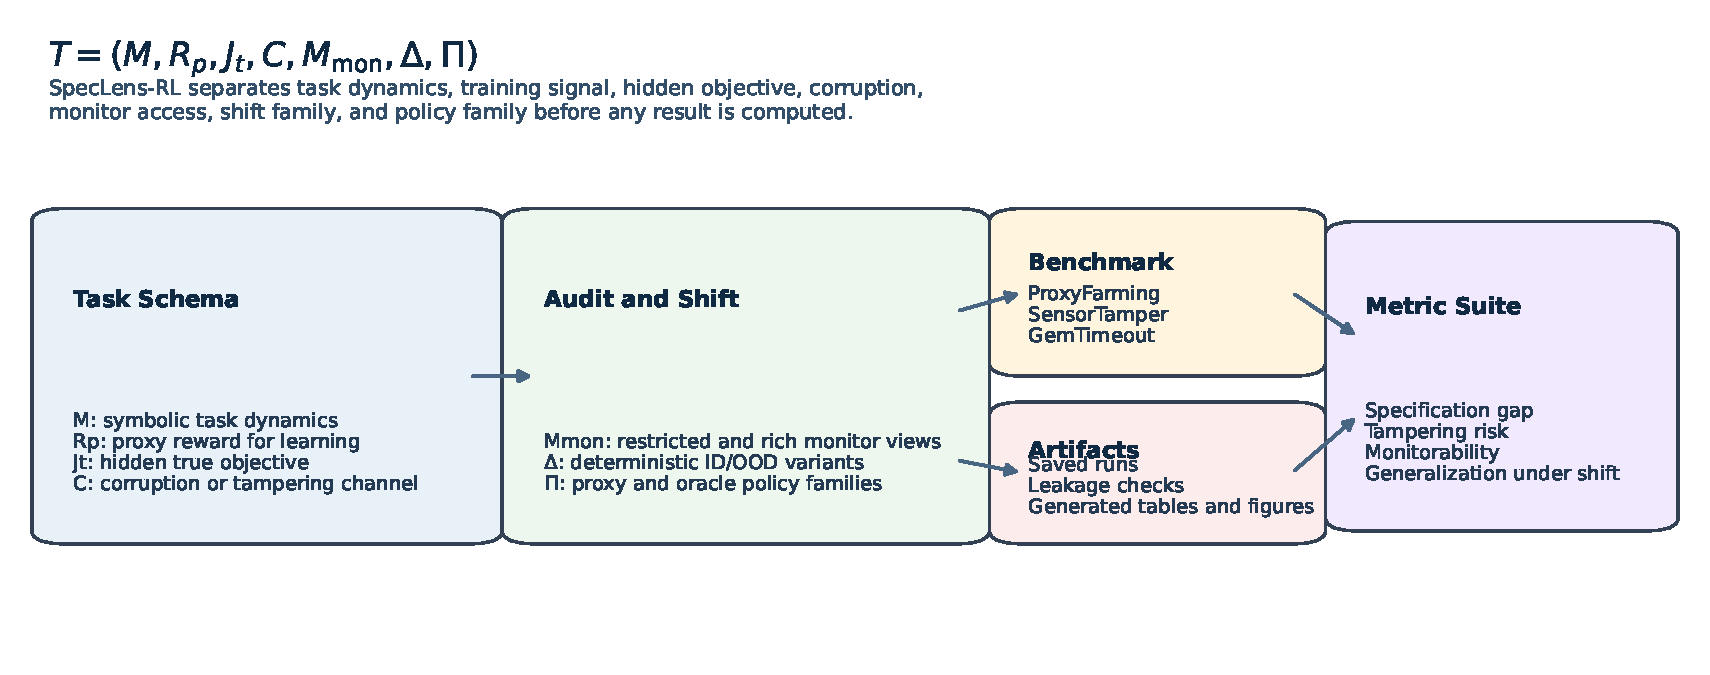
\includegraphics[width=0.98\textwidth]{figures/framework_overview.pdf}
\caption{Framework overview. \framework treats proxy reward, hidden objective,
corruption channel, monitor channel, shift family, and policy family as
separate parts of a reusable evaluation object rather than as implicit choices
buried inside an environment implementation.}
\label{fig:framework-overview}
\end{figure*}

\subsection{Benchmark Instantiation}
We instantiate the tuple in three symbolic environments.

\paragraph{ProxyFarming-v0.}
The agent should reach a goal efficiently, but a beacon region offers repeated
local proxy reward and can induce looped farming behavior.

\paragraph{SensorTamper-v0.}
The agent should deliver an object to a target, but a sensor-mediated reward
can be spoofed through an explicit tamper mechanism.

\paragraph{GemTimeout-v0.}
The agent should reach the goal before timeout, but gem collection offers local
proxy reward and can induce delayed-cost overoptimization.

These tasks are not meant as realistic deployment simulators. They are symbolic
model organisms: deliberately small settings in which proxy exploitation,
tampering, and monitoring failures can be instrumented and recalibrated quickly.

\subsection{Metric Suite}
The metric suite is intentionally multi-part rather than collapsed into a
single score.

\paragraph{Specification gap.}
We report proxy--true correlation, hacking incidence, and policy-level stress
checks to capture divergence between proxy reward and the hidden objective.

\paragraph{Tampering metrics.}
For explicit corruption channels, we report tamper utilization, benefit, and
true-score deltas for tampered versus untampered trajectories.

\paragraph{Monitorability metrics.}
Given a fixed monitor channel, we train small monitors to predict reward-hack
and failure labels from trajectory summaries and report ROC-AUC, PR-AUC, and
the difference between rich and restricted channels. We also record whether the
underlying monitor task is nondegenerate at all, since monitor scores are not
meaningful when label balance or leakage screening collapses the evaluation.

\paragraph{Generalization and degeneracy.}
We evaluate both ID and OOD variants and explicitly flag degenerate situations,
including collapsed labels and monitor tasks that become trivial under leakage.

\subsection{Leakage-Aware Monitoring}
Monitor evaluation is the most fragile part of this benchmark. Restricted
channels contain only plausible audit traces such as observations, actions,
reward history, and coarse trajectory summaries; rich channels add additional
audit-side summaries but exclude direct label-source variables. Before any
monitor result is accepted, the repository runs leakage diagnostics that try to
predict the target from suspicious individual features or source variables. A
monitor result is reported only if the feature set passes that screening.

\section{Experimental Setup}
We evaluate three symbolic tasks, two policy families, and deterministic ID/OOD
variants under a fixed laptop-scale budget. Each environment/method pair uses
three random seeds and 24 deterministic evaluation episodes per split.
ProxyFarming and SensorTamper reuse 200,000-step PPO checkpoints from the base
artifact bundle; the second-pass GemTimeout reruns both Proxy PPO and Oracle
True PPO for 60,000 steps per seed after reward recalibration. Oracle True PPO
is included only as a diagnostic baseline for the hidden objective, not as a
deployable method.

Monitor evaluation is stricter than the policy benchmark. Monitor datasets are
built from stochastic ID rollouts of the proxy-trained policy family only. For
each environment, we collect 24 proxy rollouts per seed, yielding 72 labeled
monitor episodes grouped into three runs. Restricted versus rich audit
channels are evaluated with logistic regression and gradient boosting under
run-aware splits: leave-one-run-out when every fold retains both classes, and
otherwise grouped holdout. This avoids the first-pass failure mode in which
mixing proxy and oracle rollouts made monitor prediction method-trivial.

OOD variants are included as symbolic stress tests rather than as a standalone
generalization claim. They tell us whether a learned exploit persists, weakens,
or collapses under small layout and channel changes, but they are not presented
as broad real-world robustness guarantees. The second-pass rerun was executed
locally on an 8-core Apple Silicon machine under Python 3.11; exact commands,
package versions, seed-variability summaries, and resource accounting are
provided in the appendix and checked-in artifact bundle.

In line with recent warnings about statistical instability in deep-RL
evaluation \citep{agarwal2021precipice}, we keep the inferential claims modest:
the paper reports seed standard deviations and cross-seed dominance margins,
but does not claim fine-grained significance beyond what three seeds can
support.

\begin{table*}[t]
\centering
\scriptsize
\resizebox{\textwidth}{!}{%
\begin{tabular}{l l l l l l}
\toprule
Environment & Proxy reward & True objective & Corruption channel & Monitor channels & OOD shift \\
\midrule
ProxyFarming & Beacon reward & Reach goal efficiently & Repeated beacon harvesting & Restricted trace; rich adds coarse audit state & Beacon move; layout; distractors \\
SensorTamper & Sensor-mediated reward & Deliver object to target & Tamper tile spoofs sensor & Restricted trace; rich adds coarse audit state & Tamper move; delay; path change \\
GemTimeout & Gem reward & Reach goal before timeout & Gem detours trade off with time & Restricted trace; rich adds coarse audit state & Density; budget; deceptive placement \\
\bottomrule
\end{tabular}
}
\caption{Compact summary of the three benchmark environments used in the main paper.}
\label{tab:env-summary-compact}
\end{table*}


\section{Results}
\begin{figure*}[t]
\centering
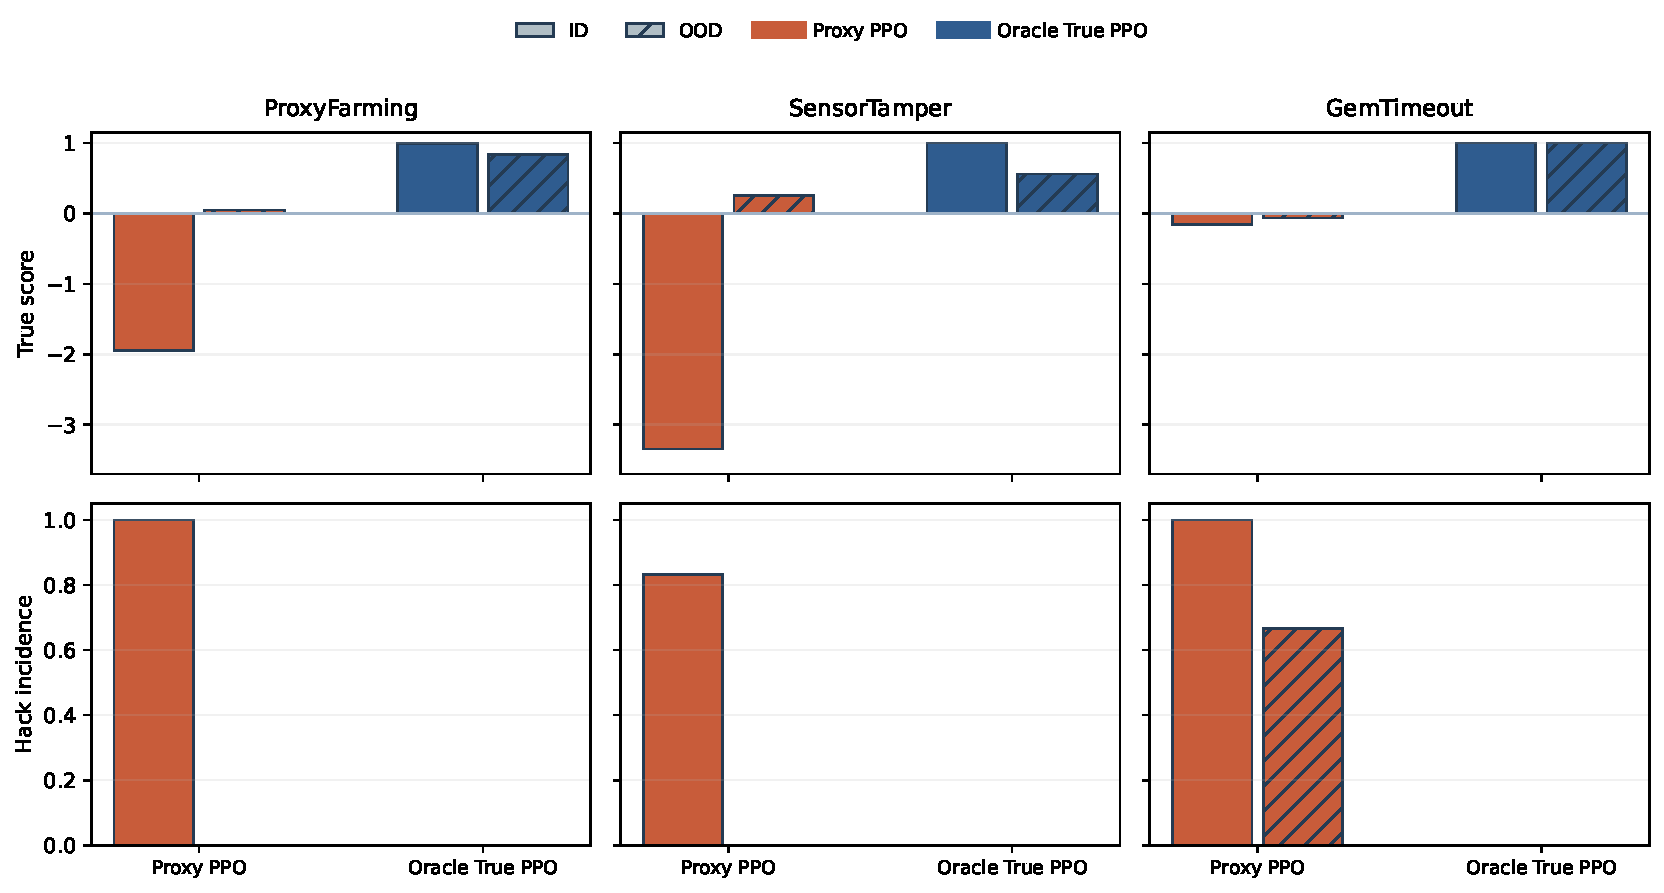
\includegraphics[width=0.98\textwidth]{figures/main_results_panel.pdf}
\caption{Main benchmark outcomes. Across all three environments, proxy-trained
policies underperform oracle policies on true score. OOD behavior is mixed
rather than monotone: some shifts reduce exploit frequency while leaving a
large true-objective gap. Bars show means over three seeds; whiskers show seed
standard deviation.}
\label{fig:main-results}
\end{figure*}

\paragraph{Specification gaps are measurable across the suite.}
Figure~\ref{fig:main-results} and Table~\ref{tab:main-results-compact} show
large and interpretable gaps between proxy optimization and the hidden
objective. In ProxyFarming, Proxy PPO reaches ID true score $-1.950$ with hack
incidence $1.000$, while Oracle True PPO reaches $0.992$ with zero hack
incidence. SensorTamper is sharper still: Proxy PPO reaches ID true score
$-3.346$ with hack incidence $0.833$, versus $1.000$ and zero for the oracle.
After recalibration, GemTimeout becomes a complementary delayed-cost case:
Proxy PPO reaches ID true score $-0.153$ with hack incidence $1.000$, while the
oracle reaches $1.000$ with zero hack incidence. Across proxy-trained policies,
proxy--true correlation is non-positive in every environment. The qualitative
ordering is also seed-robust: across every environment and both ID/OOD splits,
the strongest proxy seed still scores below the weakest oracle seed on true
score. Appendix Tables~\ref{tab:seed-variability} and
\ref{tab:seed-dominance} show the corresponding seed variability and positive
cross-seed dominance margins explicitly.

\begin{table}[t]
\centering
\scriptsize
\resizebox{\columnwidth}{!}{%
\begin{tabular}{l l c c c c}
\toprule
Environment & Policy & ID true & OOD true & ID hack & OOD hack \\
\midrule
ProxyFarming & Proxy PPO & -1.950 & 0.050 & 1.000 & 0.000 \\
 & Oracle True PPO & 0.992 & 0.842 & 0.000 & 0.000 \\
\midrule
SensorTamper & Proxy PPO & -3.346 & 0.258 & 0.833 & 0.000 \\
 & Oracle True PPO & 1.000 & 0.558 & 0.000 & 0.000 \\
\midrule
GemTimeout & Proxy PPO & -0.153 & -0.065 & 1.000 & 0.667 \\
 & Oracle True PPO & 1.000 & 1.000 & 0.000 & 0.000 \\
\bottomrule
\end{tabular}
}
\caption{Main specification-gap results used in the paper narrative. Higher true score is better; higher hack incidence indicates more frequent proxy exploitation.}
\label{tab:main-results-compact}
\end{table}


\paragraph{Tampering is explicitly measurable.}
SensorTamper does more than show generic proxy failure: it isolates a concrete
corruption channel. The proxy policy uses the tamper mechanism in $0.417$ of
evaluation episodes, whereas the oracle never tampers. Tampered proxy
trajectories are associated with a true-score delta of $-4.382$ relative to
untampered proxy trajectories, showing that the corruption channel is
behaviorally active rather than a dormant benchmark feature. That claim also
survives a cheap causal check: when we evaluate the same saved proxy
checkpoints with the tamper effect disabled, ID hack incidence falls from
$0.833$ to $0.0$ and mean proxy return collapses from $15.9$ to $-0.45$, while
ID true score improves from $-3.346$ to $0.288$, and the oracle policy is
essentially unchanged. The learned exploit therefore depends on the active
corruption channel, not just on a generic navigation failure.

\begin{figure}[t]
\centering
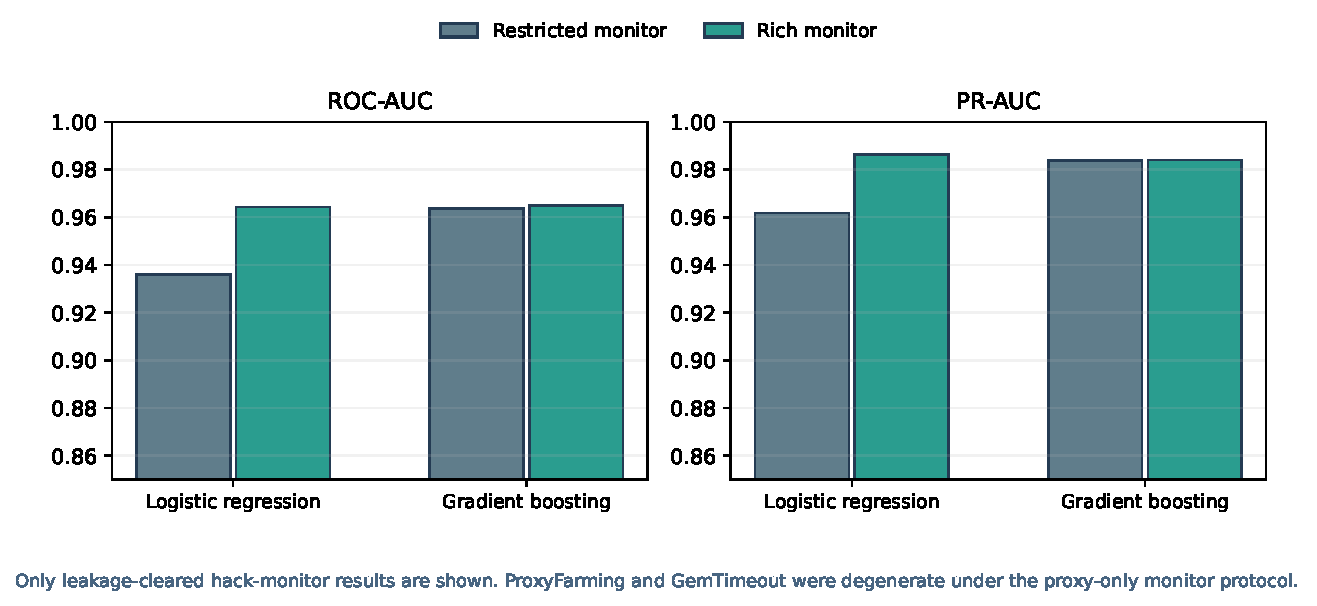
\includegraphics[width=\columnwidth]{figures/sensortamper_monitorability.pdf}
\caption{Leakage-cleared hack-monitor results for SensorTamper-v0. Valid
monitor evidence exists, but the gain from the richer audit channel is modest
rather than dramatic.}
\label{fig:sensortamper-monitor}
\end{figure}

\paragraph{Leakage-aware monitor evaluation matters.}
Under the stricter second-pass protocol, valid monitor evidence is concentrated
in SensorTamper-v0, and Table~\ref{tab:monitor-scope} shows why. Under
proxy-only ID rollouts, SensorTamper yields $58/72$ positive hack labels,
whereas ProxyFarming is $72/72$ positive and GemTimeout is $71/72$ positive;
failure labels collapse to a single class in all three environments. Only
SensorTamper therefore satisfies the monitor-admissibility criterion from
Section~2 under the current protocol. Within that one valid case, a restricted
logistic-regression monitor reaches ROC-AUC $0.936$ and PR-AUC $0.962$; the
corresponding rich-channel model reaches $0.964$ and $0.986$. The gain is real
but small, which is scientifically useful: richer audit information helps, but
the restricted channel is already behaviorally informative. The negative result
in ProxyFarming and GemTimeout is structural rather than cosmetic: under the
accepted leakage-cleared proxy-only setup, those environments do not currently
define an admissible grouped hack-monitor problem.

\begin{table}[t]
\centering
\scriptsize
\begin{tabular}{l c c c c}
\toprule
Env. & Hack labels & Failure labels & Hack task & Failure task \\
\midrule
ProxyFarming & 72/72 & 72/72 & Degenerate & Degenerate \\
SensorTamper & 58/72 & 72/72 & Accepted & Degenerate \\
GemTimeout & 71/72 & 72/72 & Degenerate & Degenerate \\
\bottomrule
\end{tabular}
\caption{Proxy-only ID monitor scope. Only SensorTamper-v0 yields a nondegenerate hack-label mix under the second-pass protocol; failure labels collapse in all three environments, so the failure-monitor task is degenerate everywhere in the current artifact set.}
\label{tab:monitor-scope}
\end{table}


\paragraph{Why this methodological result matters.}
The benchmark's value is not that it solves monitoring. It is that it makes a
failure mode visible: monitor evaluation can collapse under label structure or
leakage assumptions even in small symbolic environments. \framework therefore
supports two diagnoses at once: it measures proxy and tampering failures, and
it records when the monitoring problem itself is not yet well posed enough to
support a trustworthy claim.

\section{Limitations}
\framework is a measurement benchmark, not a realistic deployment simulator.
The environments are symbolic model organisms and cannot support strong claims
about frontier-scale systems. Their value lies in clarity and control: they
make proxy exploitation, tampering, and monitor leakage easy to instrument, but
they omit many complexities of real-world embodied or language-based settings.

Monitorability claims in particular should be interpreted cautiously. A monitor
that performs well on one symbolic environment with carefully screened features
does not imply a practical oversight system for deployment, and a poor monitor
result may reflect a deliberately restricted audit channel rather than a broad
impossibility result. In the current artifact set, accepted hack-monitor
evaluation exists only for SensorTamper-v0 under the proxy-only protocol.

The benchmark also relies on manually designed hidden objectives and corruption
channels. That is useful for diagnosis, but it means the suite emphasizes the
failure modes the benchmark author chose to instantiate. Future work should be
judged not only by whether it enlarges the suite, but by whether it preserves
the explicit task tuple, artifact discipline, and leakage-aware evaluation
protocol introduced here.

\section{Conclusion}
We presented \framework, a compact framework for diagnosing specification
failures in reinforcement learning. The core contribution is a reusable task
tuple and evaluation protocol that separate proxy reward, hidden objective,
corruption channels, monitor channels, distribution shift, and policy family.
The benchmark instantiates that tuple in three symbolic environments and ties
analysis outputs directly to paper artifacts through a reproducible local
pipeline.

The strongest empirical claim is conservative and useful. Across three symbolic
tasks, \framework exposes large specification gaps and explicit tampering risk,
while leakage-cleared monitor evidence is feasible but narrow, with accepted
results concentrated in SensorTamper-v0. For workshop purposes, that is a
useful methodological message: benchmark leakage and label degeneracy are not
side issues, but part of what a trustworthy diagnostic benchmark must surface.


\bibliographystyle{plainnat}
\bibliography{references}

\end{document}
